\appendix
\makeatletter
\renewcommand\@seccntformat[1]{\ifnum\pdfstrcmp{#1}{section}=0 Apêndice~\csname the#1\endcsname~--~\else\csname the#1\endcsname\quad\fi}
\makeatother
\renewcommand{\thetable}{\Alph{section}.\arabic{table}}
\renewcommand{\thefigure}{\Alph{section}.\arabic{figure}}
\makeatletter\@addtoreset{table}{section}\@addtoreset{figure}{section}\makeatother

\section{Regras de negócio da aplicação de referência}
\label{ap:regras}

A Tabela~\ref{tab:regras} resume as 20 regras do \texttt{SPEC.md} por módulo, e a Figura~\ref{fig:estados} mostra as transições de status da reserva.

\begin{table}[H]
\centering
\caption{Módulos e regras de negócio da aplicação de referência.}
\label{tab:regras}
\small
\begin{tabularx}{\textwidth}{@{}l l Y@{}}
\toprule
Módulo & Regras & Conteúdo \\
\midrule
Eventos & R1, R2 & Capacidade $> 0$ e nome não vazio; só eventos \texttt{ATIVO} aceitam reservas, itens e confirmações. \\
Lotes & R3--R5 & Preço $\ge 0$ e quantidade $> 0$; soma das quantidades dos lotes $\le$ capacidade do evento; $0 \le$ disponível $\le$ total. \\
Reservas & R6--R8 & Reserva nasce \texttt{CRIADA}; itens só em reserva \texttt{CRIADA}, com quantidade $> 0$ e lote do mesmo evento; subtotal $= \sum$ preço $\times$ quantidade. \\
Cupons & R9--R13 & Percentual em [1, 100] ou fixo $> 0$; desconto $= \lfloor$subtotal $\times$ \%$/100\rfloor$ ou valor fixo, limitado ao teto; desconto zero se o cupom não existe, expirou ou o subtotal está abaixo do mínimo; $0 \le$ desconto $\le$ subtotal. \\
Disponibilidade & R14--R17 & Confirmar exige itens e evento ativo; verifica todos os lotes antes de baixar qualquer um (tudo ou nada); cancelar ou expirar reserva confirmada devolve as quantidades. \\
Status & R18--R20 & Transições da Figura~\ref{fig:estados}; estados finais não mudam; entidade inexistente gera erro de ``não encontrado''. \\
\bottomrule
\end{tabularx}
\end{table}

\begin{figure}[H]
\centering
\begin{tikzpicture}[
  estado/.style={draw, rounded corners=4pt, minimum width=2.3cm, minimum height=0.8cm, font=\small},
  final/.style={estado, double},
  seta/.style={-{Stealth[length=2mm]}, thick},
  rot/.style={font=\scriptsize, inner sep=2pt}]
  \node[estado] (criada) at (0,0) {CRIADA};
  \node[estado] (confirmada) at (5,0) {CONFIRMADA};
  \node[final] (paga) at (9.2,0) {PAGA};
  \node[final] (cancelada) at (2.5,-1.6) {CANCELADA};
  \node[final] (expirada) at (2.5,-3.0) {EXPIRADA};
  \draw[seta] (criada) -- node[rot, above] {confirmar} (confirmada);
  \draw[seta] (confirmada) -- node[rot, above] {pagar} (paga);
  \draw[seta] (criada.south east) -- node[rot, above right, pos=0.4] {cancelar} (cancelada.north west);
  \draw[seta] (confirmada.south west) -- node[rot, above left, pos=0.4] {cancelar$^{*}$} (cancelada.north east);
  \draw[seta] (criada.south) |- node[rot, left, pos=0.4] {expirar} (expirada.west);
  \draw[seta] (confirmada.south) |- node[rot, right, pos=0.4] {expirar$^{*}$} (expirada.east);
\end{tikzpicture}
\caption{Transições de status da reserva (R18). Estados com borda dupla são finais (R19). $^{*}$Devolve a disponibilidade dos lotes (R17).}
\label{fig:estados}
\end{figure}

\section{Propriedades das suítes}
\label{ap:propriedades}

A Tabela~\ref{tab:propriedades} lista as 17 propriedades, as regras que cada uma verifica e o tipo de oráculo. O enunciado completo e as faixas dos geradores estão no \texttt{SPEC.md}.

\begin{table}[H]
\centering
\caption{Propriedades, regras verificadas e tipo de oráculo. P1--P8 formam a suíte fraca; P1--P17, a suíte forte.}
\label{tab:propriedades}
\small
\begin{tabularx}{\textwidth}{@{}L{3.4cm} Y l l@{}}
\toprule
Propriedade & Enunciado & Regras & Oráculo \\
\midrule
P1 Total não negativo & Para qualquer reserva e cupom, total $\ge 0$ & R8, R11--R13 & limite \\
P2 Desconto limitado & $0 \le$ desconto $\le$ subtotal e total $=$ subtotal $-$ desconto & R11, R13 & limite \\
P3 Comutatividade & Permutar os itens não altera o subtotal & R8 & metamórfico \\
P4 Cupom inválido neutro & Cupom inexistente, expirado ou abaixo do mínimo não altera o total & R12 & neutralidade \\
P5 Disponibilidade não negativa & Após confirmações, $0 \le$ disponível $\le$ total & R5, R15 & limite \\
P6 Redução correta & Confirmação aceita reduz exatamente o pedido; recusada não altera lotes & R15, R16 & valor exato \\
P7 Cancelamento restaura & Confirmar e cancelar (ou expirar) devolve a disponibilidade inicial & R17 & ida e volta \\
P8 Transições válidas & Sequências de operações seguem a Figura~\ref{fig:estados} ou são recusadas sem efeito & R18, R19 & modelo \\
\midrule
P9 Oráculo de preço & Subtotal, desconto e total iguais aos do modelo & R8, R11--R13 & modelo \\
P10 Validação de evento & Evento inválido é recusado; válido nasce \texttt{ATIVO} com os mesmos dados & R1, R2 & valor exato \\
P11 Lote e capacidade & Cada cadastro de lote é aceito ou recusado exatamente como no modelo de capacidade & R3--R5 & modelo \\
P12 Validação de cupom & O cadastro aceita exatamente os cupons válidos e preserva os dados & R9 & valor exato \\
P13 Itens da reserva & Adicionar item segue a ordem de verificação e registra o item aceito & R7 & valor exato \\
P14 Evento inativo e reserva vazia & Só evento ativo aceita reservas, itens e confirmações; reserva vazia não confirma & R2, R6, R14 & valor exato \\
P15 Cupom em reserva criada & Aplicar cupom só em reserva \texttt{CRIADA}; nos demais status, recusa sem efeito & R10 & valor exato \\
P16 Entidade inexistente & Toda operação sobre id inexistente falha com o código da entidade & R20 & valor exato \\
P17 Modelo de estoque & Estoque, status e erros iguais aos do modelo após cada operação de uma sequência & R15--R19 & modelo \\
\bottomrule
\end{tabularx}
\end{table}

\section{Operadores de mutação e decisões de projeto do experimento}
\label{ap:operadores}

O PIT foi executado com a união dos grupos \texttt{DEFAULTS}, \texttt{STRONGER} e do operador \texttt{NEGATE\_CONDITIONALS}; o StrykerJS, com seu conjunto padrão. Sobre os mesmos resultados, dois recortes são calculados por mutante, o que é válido porque cada mutante é avaliado isoladamente:

\begin{itemize}
  \item \textbf{Padrão}: o conjunto padrão de cada ferramenta, como um desenvolvedor a usaria (\texttt{DEFAULTS} no PIT 1.18; todos os operadores no StrykerJS).
  \item \textbf{Harmonizado}: apenas as cinco classes de mutação que existem com a mesma transformação nas duas ferramentas (Tabela~\ref{tab:categorias}). O operador de igualdade do StrykerJS foi dividido em limite (\texttt{<} $\leftrightarrow$ \texttt{<=}) e negação (\texttt{===} $\to$ \texttt{!==}, \texttt{<} $\to$ \texttt{>=}) conforme o operador original e o substituto.
\end{itemize}

\begin{table}[H]
\centering
\caption{Classes de mutação do recorte harmonizado. Ficam fora do recorte os operadores sem equivalente: valores de retorno e remoção de chamadas no PIT; literais, blocos, chamadas de método e operadores lógicos no StrykerJS.}
\label{tab:categorias}
\small
\begin{tabularx}{\textwidth}{@{}l Y Y@{}}
\toprule
Classe & PIT & StrykerJS \\
\midrule
Aritmético & \texttt{Math}, \texttt{InvertNegs} & \texttt{ArithmeticOperator}, \texttt{AssignmentOperator}, \texttt{UnaryOperator} \\
Limite relacional & \texttt{ConditionalsBoundary} & \texttt{EqualityOperator} (\texttt{<}$\leftrightarrow$\texttt{<=}, \texttt{>}$\leftrightarrow$\texttt{>=}) \\
Negação relacional & \texttt{NegateConditionals} & \texttt{EqualityOperator} (demais substituições) \\
Condição forçada & \texttt{RemoveConditional} (\texttt{EQUAL}/\texttt{ORDER}, \texttt{IF}/\texttt{ELSE}) & \texttt{ConditionalExpression} \\
Incremento & \texttt{Increments} & \texttt{UpdateOperator} \\
\bottomrule
\end{tabularx}
\end{table}

As demais decisões de projeto do experimento foram:

\begin{itemize}
  \item \textbf{Mutação só no domínio.} PIT e StrykerJS mutam apenas a camada de domínio; controladores e configuração do framework não contêm regra de negócio.
  \item \textbf{Propriedades chamam o domínio diretamente}, não via HTTP, para que o tempo medido não inclua o custo de cada servidor web.
  \item \textbf{Dinheiro em centavos inteiros} nos dois lados, evitando divergências de ponto flutuante que não são do ecossistema.
  \item \textbf{Configurações equivalentes:} geração aleatória e semente nova a cada execução nos dois lados. No jqwik, o reaproveitamento da semente que falhou na execução anterior foi desligado, para que um mutante não influencie o próximo. O número de tentativas é passado às duas bibliotecas por configuração (\texttt{jqwik.tries.default} e \texttt{numRuns}).
  \item \textbf{Matriz completa de mortes:} o PIT registra todos os testes que matam cada mutante (\textit{full mutation matrix}) e o StrykerJS não para no primeiro teste que falha (\texttt{disableBail}), o que permite atribuir cada morte a uma ou mais propriedades.
  \item \textbf{Ordem aleatória:} em cada uma das 30 rodadas, as 12 configurações foram executadas em ordem aleatória (semente = número da rodada), para que variações de carga da máquina não se concentrem em uma configuração.
\end{itemize}

\section{Figuras complementares}
\label{ap:figuras}

\begin{figure}[H]
\centering
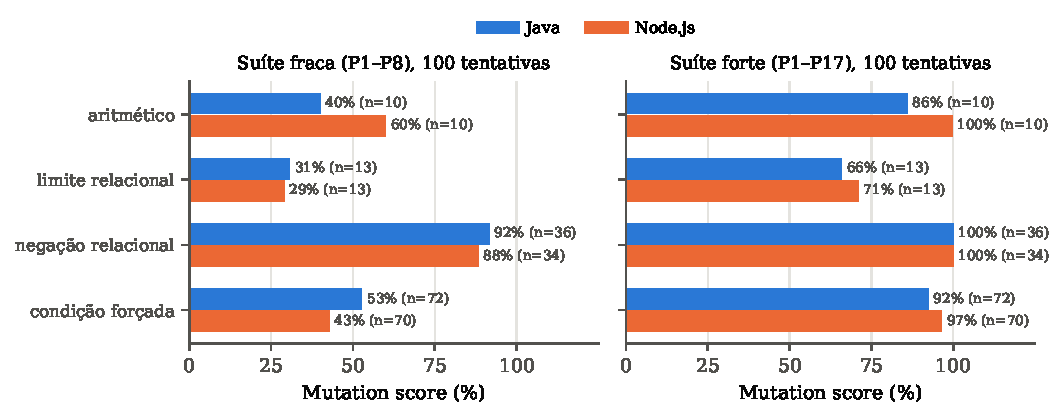
\includegraphics[width=\textwidth]{figuras/fig5_2_classes_harmonizadas.pdf}
\caption{\textit{Mutation score} por classe de mutação do recorte harmonizado (100 tentativas). Entre parênteses, o número de mutantes da classe por execução. A classe incremento, com um único mutante no Node.js, foi omitida.}
\label{fig:classes}
\end{figure}

\begin{figure}[H]
\centering
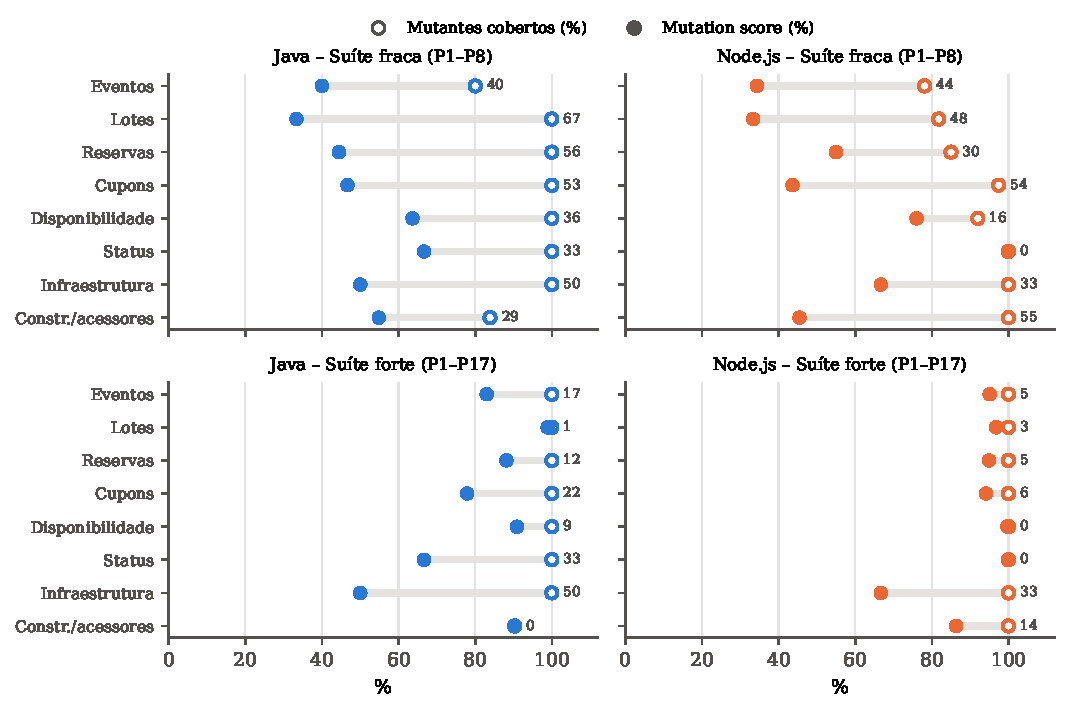
\includegraphics[width=\textwidth]{figuras/fig5_3_cobertura_vs_score.pdf}
\caption{Mutantes cobertos pela suíte $\times$ \textit{mutation score}, por módulo (100 tentativas, operadores padrão). O rótulo à direita é a diferença em pontos percentuais (QP5).}
\label{fig:cobertura}
\end{figure}

\begin{figure}[H]
\centering
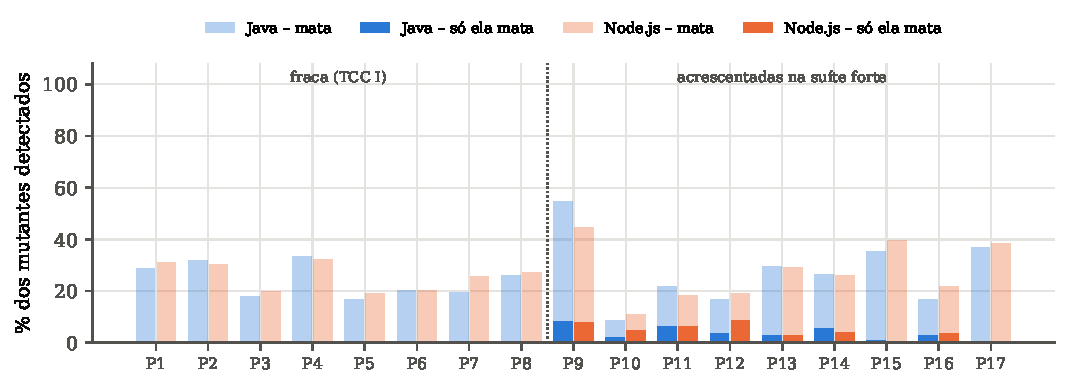
\includegraphics[width=\textwidth]{figuras/fig5_4_mortos_por_propriedade.pdf}
\caption{Suíte forte, 100 tentativas: porcentagem dos mutantes detectados que cada propriedade mata (clara) e que só ela mata (escura), média por execução (QP6).}
\label{fig:propriedades}
\end{figure}

\begin{figure}[H]
\centering
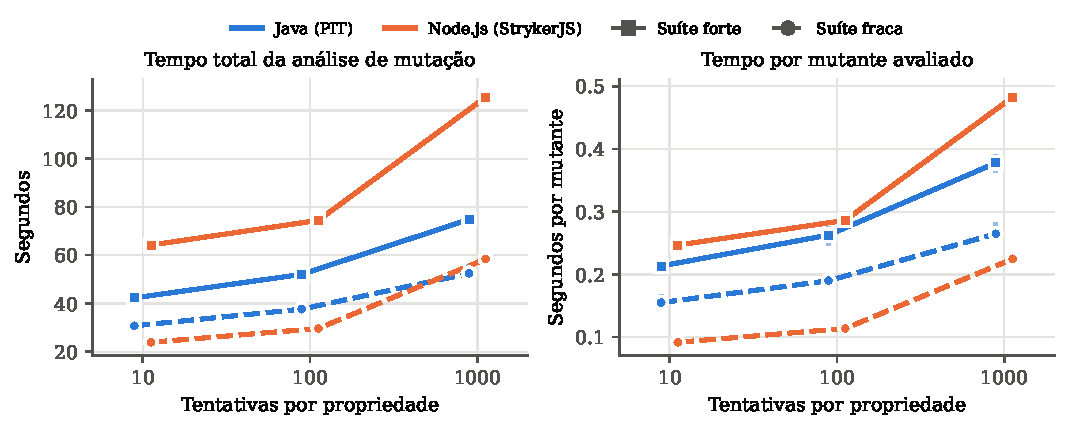
\includegraphics[width=\textwidth]{figuras/fig5_5_tempo.pdf}
\caption{Tempo da análise de mutação, total e por mutante avaliado: mediana (marcador) e intervalo interquartil (barra) das 30 execuções (QP7).}
\label{fig:tempo}
\end{figure}

\section{Testes estatísticos complementares}
\label{ap:testes}

Além de $H_0$, os efeitos da suíte, do número de tentativas e o tempo foram comparados com o mesmo procedimento (Mann-Whitney U bilateral, $n = 30$ por grupo, $\hat{A}_{12}$ e $p$ corrigido por Holm sobre os 38 testes do estudo). Essas comparações descrevem os fatores controlados e não constituem hipóteses adicionais. Na Tabela~\ref{tab:testes-compl}, $\hat{A}_{12}$ é a probabilidade de uma execução do primeiro grupo superar uma do segundo.

\begin{table}[H]
\centering
\caption{Comparações complementares. A última coluna indica se a igualdade foi rejeitada a $\alpha = 0{,}05$.}
\label{tab:testes-compl}
\small
\begin{tabular*}{\textwidth}{@{\extracolsep{\fill}}l l l r r l@{}}
\toprule
Comparação & Contexto & Grupos & $\hat{A}_{12}$ & $p$ & Igualdade \\
\midrule
Suíte & Java, 10 tent. & forte $\times$ fraca & \aumSuiteJavaDez & \pSuiteJavaDez & \decSuiteJavaDez \\
Suíte & Java, 100 tent. & forte $\times$ fraca & \aumSuiteJavaCem & \pSuiteJavaCem & \decSuiteJavaCem \\
Suíte & Java, 1000 tent. & forte $\times$ fraca & \aumSuiteJavaMil & \pSuiteJavaMil & \decSuiteJavaMil \\
Suíte & Node.js, 10 tent. & forte $\times$ fraca & \aumSuiteNodeDez & \pSuiteNodeDez & \decSuiteNodeDez \\
Suíte & Node.js, 100 tent. & forte $\times$ fraca & \aumSuiteNodeCem & \pSuiteNodeCem & \decSuiteNodeCem \\
Suíte & Node.js, 1000 tent. & forte $\times$ fraca & \aumSuiteNodeMil & \pSuiteNodeMil & \decSuiteNodeMil \\
\midrule
Tentativas & Java, fraca & 100 $\times$ 10 & \aumTentJavaFracaCem & \pTentJavaFracaCem & \decTentJavaFracaCem \\
 & & 1000 $\times$ 100 & \aumTentJavaFracaMil & \pTentJavaFracaMil & \decTentJavaFracaMil \\
Tentativas & Java, forte & 100 $\times$ 10 & \aumTentJavaForteCem & \pTentJavaForteCem & \decTentJavaForteCem \\
 & & 1000 $\times$ 100 & \aumTentJavaForteMil & \pTentJavaForteMil & \decTentJavaForteMil \\
Tentativas & Node.js, fraca & 100 $\times$ 10 & \aumTentNodeFracaCem & \pTentNodeFracaCem & \decTentNodeFracaCem \\
 & & 1000 $\times$ 100 & \aumTentNodeFracaMil & \pTentNodeFracaMil & \decTentNodeFracaMil \\
Tentativas & Node.js, forte & 100 $\times$ 10 & \aumTentNodeForteCem & \pTentNodeForteCem & \decTentNodeForteCem \\
 & & 1000 $\times$ 100 & \aumTentNodeForteMil & \pTentNodeForteMil & \decTentNodeForteMil \\
\midrule
Tempo total & fraca, 10 tent. & Java $\times$ Node.js & \aumTempoFracaDezTotal & \pTempoFracaDezTotal & \decTempoFracaDezTotal \\
Tempo/mutante & fraca, 10 tent. & Java $\times$ Node.js & \aumTempoFracaDezMutante & \pTempoFracaDezMutante & \decTempoFracaDezMutante \\
Tempo total & fraca, 100 tent. & Java $\times$ Node.js & \aumTempoFracaCemTotal & \pTempoFracaCemTotal & \decTempoFracaCemTotal \\
Tempo/mutante & fraca, 100 tent. & Java $\times$ Node.js & \aumTempoFracaCemMutante & \pTempoFracaCemMutante & \decTempoFracaCemMutante \\
Tempo total & fraca, 1000 tent. & Java $\times$ Node.js & \aumTempoFracaMilTotal & \pTempoFracaMilTotal & \decTempoFracaMilTotal \\
Tempo/mutante & fraca, 1000 tent. & Java $\times$ Node.js & \aumTempoFracaMilMutante & \pTempoFracaMilMutante & \decTempoFracaMilMutante \\
Tempo total & forte, 10 tent. & Java $\times$ Node.js & \aumTempoForteDezTotal & \pTempoForteDezTotal & \decTempoForteDezTotal \\
Tempo/mutante & forte, 10 tent. & Java $\times$ Node.js & \aumTempoForteDezMutante & \pTempoForteDezMutante & \decTempoForteDezMutante \\
Tempo total & forte, 100 tent. & Java $\times$ Node.js & \aumTempoForteCemTotal & \pTempoForteCemTotal & \decTempoForteCemTotal \\
Tempo/mutante & forte, 100 tent. & Java $\times$ Node.js & \aumTempoForteCemMutante & \pTempoForteCemMutante & \decTempoForteCemMutante \\
Tempo total & forte, 1000 tent. & Java $\times$ Node.js & \aumTempoForteMilTotal & \pTempoForteMilTotal & \decTempoForteMilTotal \\
Tempo/mutante & forte, 1000 tent. & Java $\times$ Node.js & \aumTempoForteMilMutante & \pTempoForteMilMutante & \decTempoForteMilMutante \\
\bottomrule
\end{tabular*}
\end{table}

O teste de Kruskal-Wallis entre os três níveis de tentativas rejeitou a igualdade nas quatro combinações de ecossistema e suíte (Java fraca: \kwJavaFraca; Java forte: \kwJavaForte; Node.js fraca: \kwNodeFraca; Node.js forte: \kwNodeForte). Na suíte fraca, porém, as diferenças são menores que 3 pontos percentuais (Tabela~\ref{tab:resumo}): com 30 execuções e variância quase nula, diferenças pequenas já são significativas, e por isso o tamanho do efeito e a diferença absoluta devem ser lidos junto com o $p$-valor.

\section{Ameaças à validade}
\label{ap:ameacas}

\begin{table}[H]
\centering
\caption{Ameaças à validade, mitigações adotadas e mitigações futuras.}
\label{tab:ameacas}
\small
\begin{tabularx}{\textwidth}{@{}l Y Y Y@{}}
\toprule
Validade & Ameaça & Mitigação adotada & Mitigação futura \\
\midrule
Conclusão & As 30 execuções reavaliam os mesmos mutantes; variância baixa em algumas configurações & $\hat{A}_{12}$, correção de Holm, qui-quadrado com o mutante distinto como unidade & Mais aplicações, para que a unidade amostral seja o programa \\
Conclusão & Tempo medido em máquina virtual compartilhada & Ordem aleatória das configurações em cada rodada; mediana; tempo por mutante & Repetir em máquina dedicada \\
Interna & Implementações não equivalentes & Especificação única, 11 cenários compartilhados (125 passos) aprovados nos dois lados & Testes diferenciais gerados automaticamente entre as duas APIs \\
Interna & Propriedades mais fortes em um lado & Mesmos enunciados, geradores e tentativas, mapeados 1:1 & Revisão das propriedades por um segundo pesquisador \\
Interna & Suíte forte ajustada aos mutantes & Propriedades derivadas do \texttt{SPEC.md}; ajustes do piloto declarados (Seção~\ref{sec:fluxo}) & Suíte escrita por quem não vê os mutantes \\
Interna & Ferramentas Java compiladas do código-fonte & Mesmas versões publicadas; CI com o \textit{plugin} Maven oficial reproduziu os resultados & --- \\
Construto & \textit{Mutation score} como medida de efetividade & Complementado por cobertura, análise por módulo e classificação & Usar defeitos reais injetados \\
Construto & Conjuntos de operadores diferentes entre PIT e StrykerJS & Recorte harmonizado com cinco classes de mesma transformação & Implementar operadores idênticos nas duas ferramentas \\
Construto & Classificação dos não detectados & Critérios objetivos, mapa linha--regra versionado, justificativa por mutante, revisão e confirmação pelo autor & Classificação independente com cálculo de concordância \\
Externa & Um domínio pequeno, propriedades no nível do domínio & Domínio com regras numéricas, de estado e de disponibilidade & Replicar em APIs de outros domínios, via HTTP \\
\bottomrule
\end{tabularx}
\end{table}
